\documentclass{ceurart}

\usepackage{acronym}
\usepackage{subcaption}

\renewcommand{\acffont}[1]{\textsl{#1}}


%%
%% end of the preamble, start of the body of the document source.
\begin{document}

%%
%% Rights management information.
%% CC-BY is default license.
\copyrightyear{2026}
\copyrightclause{Copyright for this paper by its authors.\\
  Use permitted under Creative Commons License Attribution 4.0
  International (CC BY 4.0).}

%%
%% This command is for the conference information
\conference{``Search Engines'', course at the master degree in ``Computer Engineering'', Department of Information Engineering, and at the master degree in ``Data Science'', Department of Mathematics ``Tullio Levi-Civita'', University of Padua, Italy. Academic Year 2025/2026}

%%
%% The "title" command
\title{SEUPD@CLEF: Team retrix on Source Retrieval for Scientific Web Claims}

%%
%% The "author" command and its associated commands are used to define
%% the authors and their affiliations.
\author[1]{Fabio Baldan}[%
email=fabio.baldan.1@studenti.unipd.it
]

\author[1]{Giancarlo Padoan}[%
email=giancarlo.padoan@studenti.unipd.it
]

\author[1]{Alvise Garberino}[%
email=alvise.garberino@studenti.unipd.it
]

\author[1]{Marco Tessari}[%
email=marco.tessari.8@studenti.unipd.it
]

\author[1]{Davide Donati}[%
email=davide.donati@studenti.unipd.it
]

\address[1]{University of Padua, Italy}



%%
%% The abstract is a short summary of the work to be presented in the
%% article.
\begin{abstract}
We present the results of the retrix group for the CheckThat! 2026 - Task 1, in which the goal is to identify the scientific paper implicitly referenced in a social media post. The input consists of short, noisy and usually informal posts that mention scientific findings without providing explicit links or explicit citations.

Our approach is designed to operate in a multilingual setting, as the dataset includes posts in English, German, and French. To handle this, we used multi-lingual language models. 

DA FINIRE CON PIPELINE FINALEEEEEE
DA FINIRE CON PIPELINE FINALEEEEEE
DA FINIRE CON PIPELINE FINALEEEEEE
DA FINIRE CON PIPELINE FINALEEEEEE
\end{abstract}


%%
%% Keywords. The author(s) should pick words that accurately describe
%% the work being presented. Separate the keywords with commas.
\begin{keywords}
  Fact Checking \sep
  Information Retrieval \sep
  Scientific Document Retrieval \sep
  Social media fact verification \sep
  CLEF \sep
  Neural Re-ranking \sep
  Cross Encoder
  
\end{keywords}

%%
%% This command processes the author and affiliation and title
%% information and builds the first part of the formatted document.
\maketitle


\section{Introduction}
\label{sec:introduction}

The rapid dissemination of scientific claims through social media poses a substantial challenge for fact-checking, as
posts frequently summarize, simplify, or sensationalize research findings while omitting an explicit reference to the
original study. As a result, the scientific source underlying a claim is rarely provided through a direct URL or a
complete bibliographic citation and is instead only hinted at through partial cues, such as the reported finding, the
publication venue, the research institution, or the authors involved, making verification not merely a matter of
assessing the plausibility of the claim itself, but first and foremost a matter of identifying the scientific
publication to which the post implicitly refers.

This problem is addressed in Task 1 of the CLEF 2026 CheckThat! Lab, \emph{Source Retrieval for Scientific Web Claims},
whose objective is to identify, for each social media post containing a scientific claim and an implicit reference to a
study, the corresponding publication within a fixed pool of 10,000 English-language candidate papers.

The task is particularly challenging because it requires bridging the marked gap between the language of social media
and that of scientific writing, as posts are typically short, informal, and often expressed through paraphrases,
slogans, hashtags, or incomplete statements, whereas scientific papers adopt a much more precise and technical register.
At the same time, the referenced source is not cited explicitly, meaning that the retrieval system cannot rely on direct
bibliographic signals and must instead infer the connection from partial semantic evidence; this challenge is further
compounded by the variety of forms in which relevant clues may appear, including mentions of a scientific finding, a
medical outcome, a research institution, or a publication venue, thus requiring the effective integration of lexical and
semantic evidence.

A further layer of complexity is introduced by the multilingual nature of the benchmark, since the official query sets
include posts in English, German, and French, while the candidate collection is shared across languages. Consequently,
an effective retrieval system must not only reconstruct the implicit link between a post and its source publication, but
must also do so in a setting where the evidence is expressed in multiple languages and must ultimately be mapped onto
the same English-language document pool.

Team Retrix addresses this task through a four-stage sequential pipeline (Figure~\ref{fig:pipeline}):
\begin{enumerate}
    \item {Queries originally written in French or German are first translated into English using
    \sloppy{utter-project/EuroLLM-9B-Instruct-2512}, so that all downstream components can operate over a unified input
    space independently of the source language.}

    \item {The resulting English queries are then enriched through a pseudo-relevance feedback strategy, where
    \sloppy{BAAI/bge-large-en-v1.5} is used to retrieve semantically related papers and extract salient expansion terms,
    thereby helping bridge the gap between the informal language of social media posts and the more specialized
    terminology of scientific publications.}

    \item {The expanded queries are subsequently processed by a hybrid retriever based on \sloppy{BAAI/bge-m3}, which
    combines dense, sparse, and ColBERT-style signals in order to generate a high-recall list of candidate papers from
    the shared collection.}

    \item {The retrieved candidates are reranked with a neural cross-encoder, with
    \sloppy{nvidia/llama-nemotron-rerank-1b-v2} providing our strongest single-stage configuration, while additional
    experiments with cascaded and fine-tuned rerankers were conducted to further improve the ordering of the top results.}
\end{enumerate}

Throughout the development of this pipeline, we also investigated the effect of fine-tuning reranking models on
domain-specific hard negatives derived from the training data. \\

%Todo : inserire il posizionamento
Evaluated on the CheckThat! 2026 Task 1 dataset our system ranked XXXXXXXXXXXXX on the official leaderboard attaining an
average Mean Reciprocal Rank at 5 (MRR@5) of XXXXXXXXXXXXXX \% on the development set (XXXXX place). \\

The remainder of this paper is organized as follows: Section~\ref{sec:related} reviews the research directions most
closely related to the task, Section~\ref{sec:methodology} presents our approach in detail, Section~\ref{sec:setup}
describes the experimental setup, and Section~\ref{sec:results} discusses the main results, while
Section~\ref{sec:conclusion} concludes the paper by summarizing our findings and outlining possible directions for
future work.


\section{Methodology}
\label{sec:methodology}

We started from a lexical baseline based on Apache Lucene BM25 and progressively moved to a multi-stage neural pipeline.
Early experiments focused on analyzer choices, stopword lists, and BM25 variants; these runs were useful to establish a stable
baseline, but they also showed that lexical overlap alone is insufficient for this task.
\newline
We adopted a four-stage pipeline (Figure~\ref{fig:pipeline}) for our information retrieval system, consisting of:
\begin{itemize}
    \item \textbf{Query Translation}: queries in French or German are first translated into English.
    \item \textbf{Query expansion}: we expanded the English query with additional context to bridge the gap between informal and domain specific language.
    \item \textbf{Retrieval}: we retrieved relevant documents from the corpus using the expanded query.
    \item \textbf{Reranking}: we reranked the retrieved documents based on their relevance to the original query.
\end{itemize}
For each of these stages, we experimented with different models, chosing the ones that performed better in relation to the others.

In the following sections all the four stages are precisely explained.

\begin{figure}
    \centering
    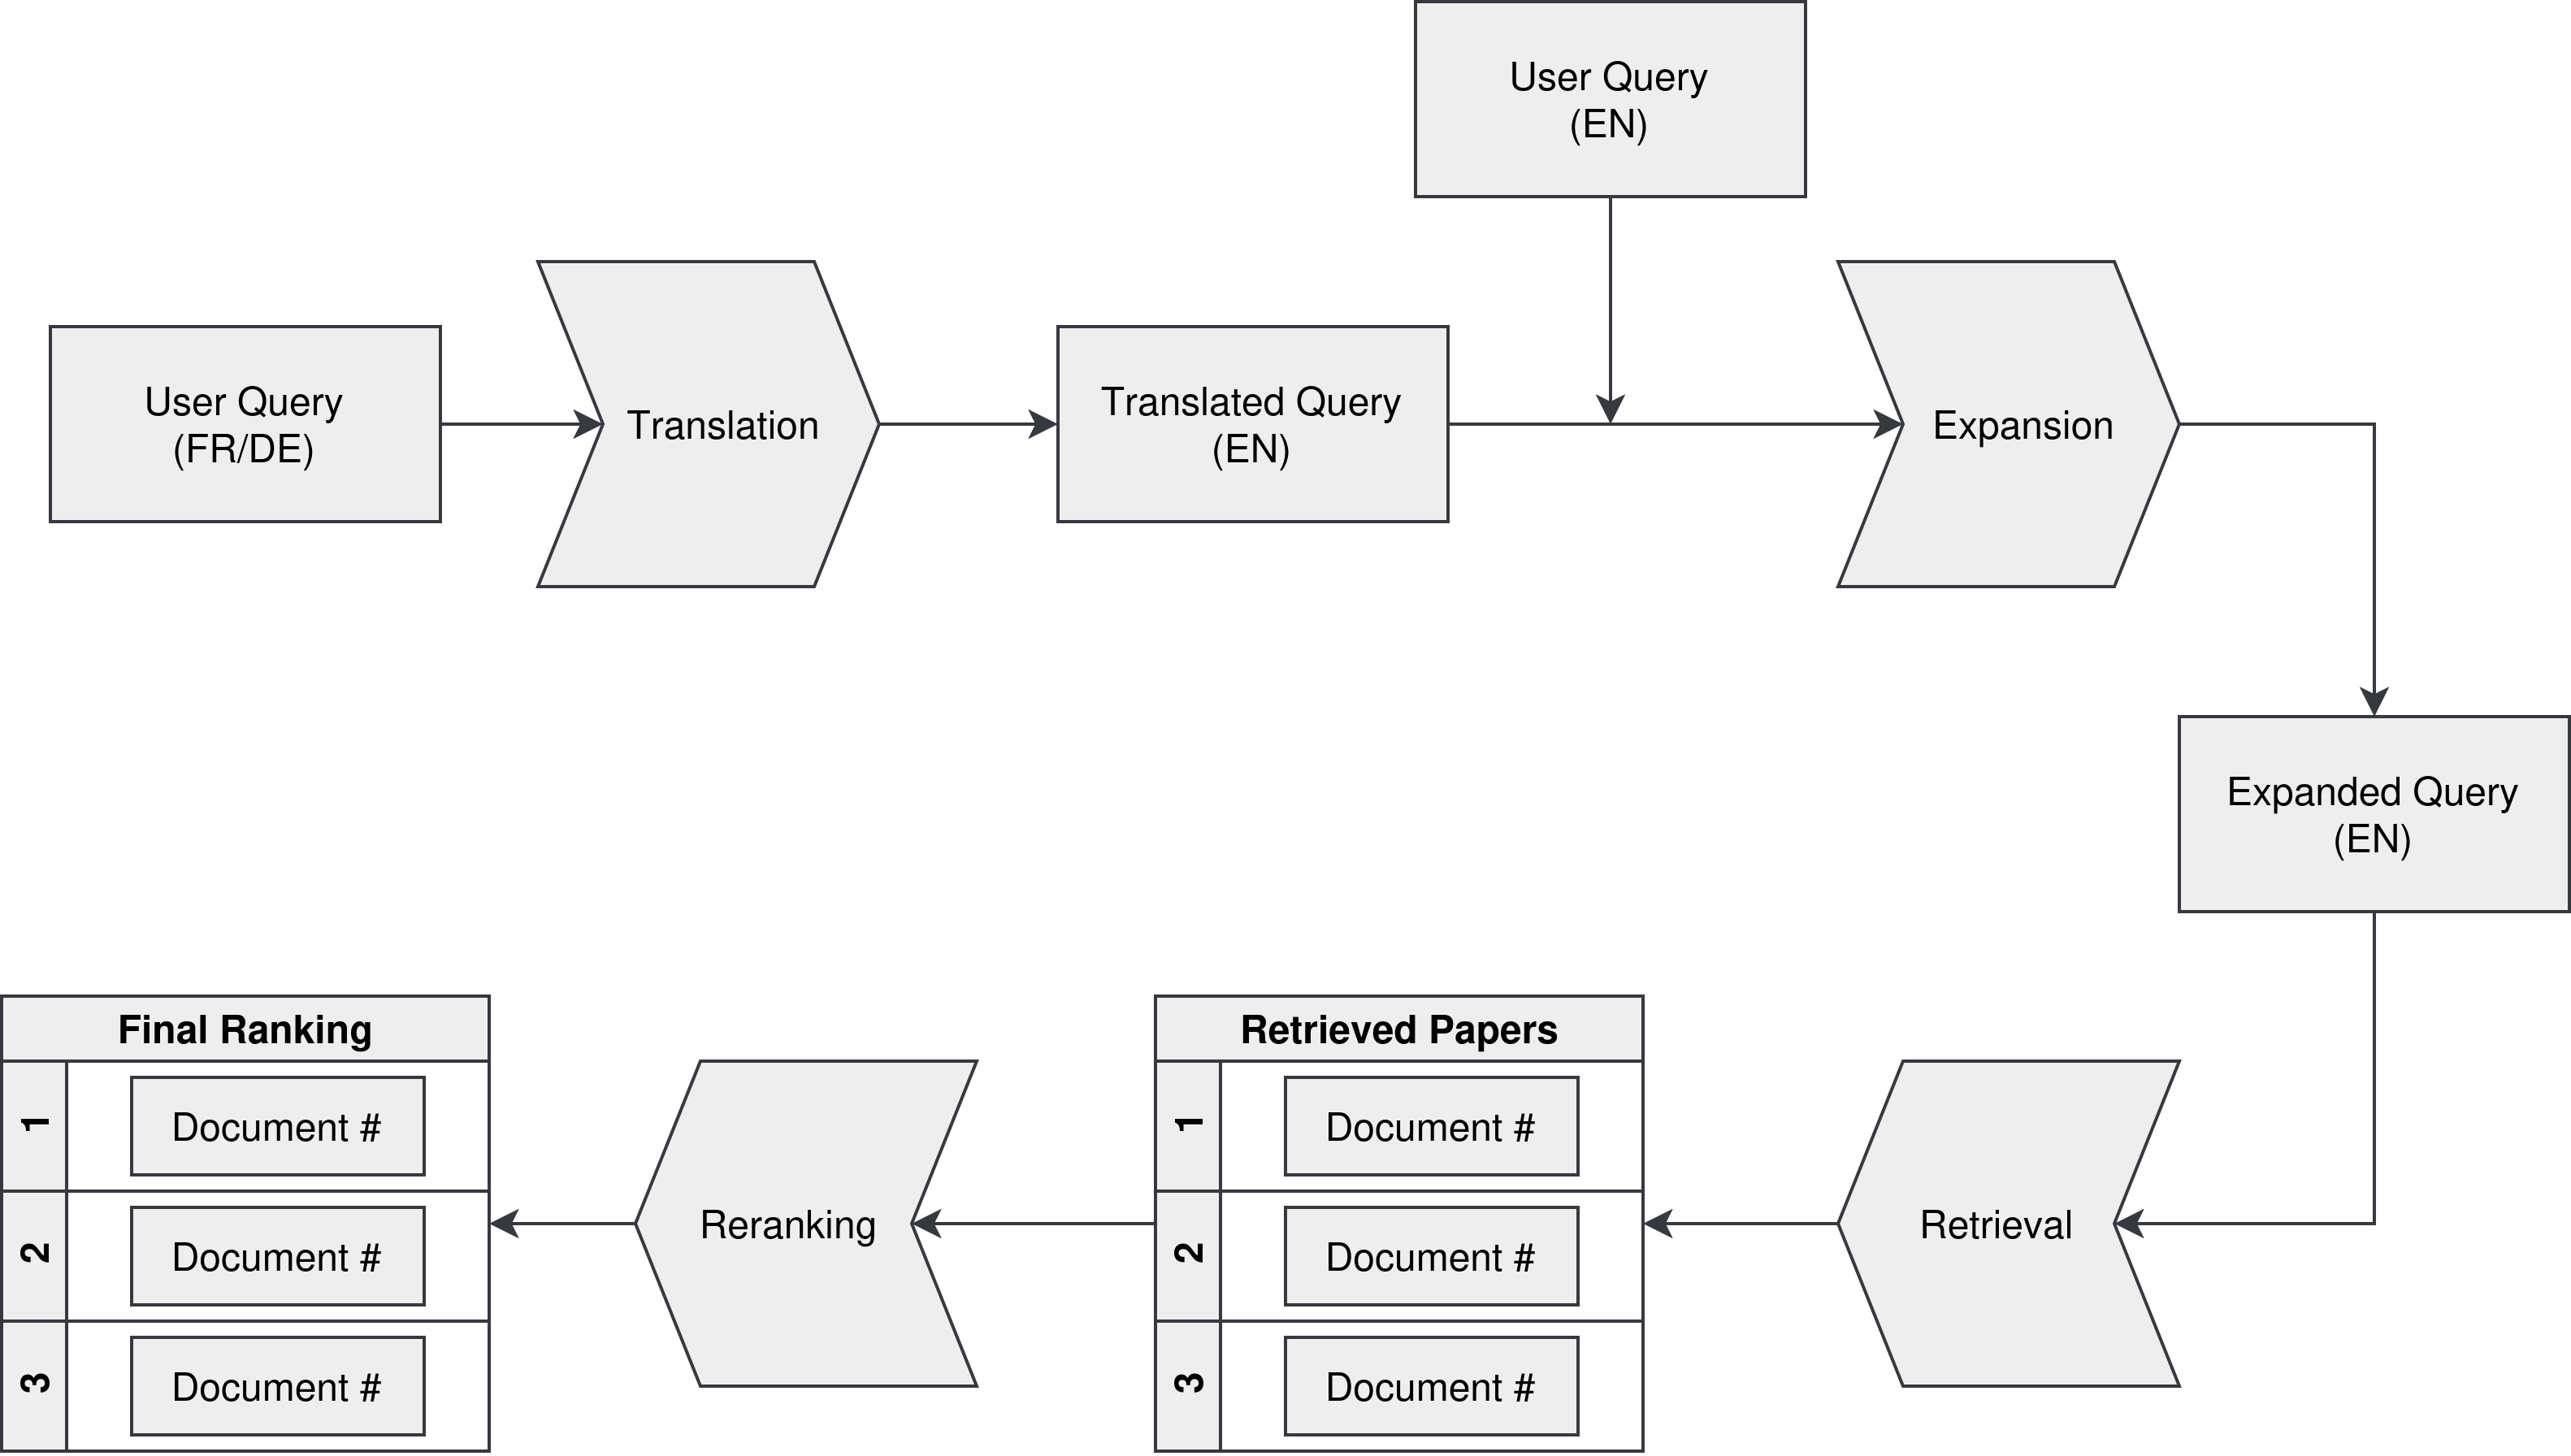
\includegraphics[width=0.8\linewidth]{figure/pipe.png}
    \caption{Four-stage pipeline for information retrieval.}
    \label{fig:pipeline}
\end{figure}

\subsection{Query translation} \label{sub:querytransl}
In the preliminary stage of out pipeline non-English queries (French and German) are translated into English. This is done query by query using the model \texttt{utter-project/EuroLLM-9B-Instruct-2512} with the following prompt:
\begin{promptbox}
\small
\ttfamily
\begin{flushleft}
\textit{system:} You are a professional translator.\\
Translate the user's text to English.\\
Output ONLY the English translation.\\
Do not include the original text, explanations, labels, or any other content.\\[0.8em]

\textit{user:} Translate this \{\textbf{French/German}\} text to English.\\
Output only the English translation, nothing else.\\[0.8em]

\{\textbf{Query original text}\}
\end{flushleft}
\end{promptbox}

The resulting English queries are then fed into the following step of our pipeline. 

\subsection{Query Expansion} \label{sub:queryexp}
Following the translation phase, the English queries undergo a semantic and lexical expansion process. This stage is designed to bridge the vocabulary gap between the user's informal query and the formal academic language present in the scientific document corpus. Unlike previous iterations that relied on generative LLM re-phrasings, the current architecture utilizes a hybrid expansion strategy, combining deep semantic retrieval with linguistic analysis. The expansion process follows three main technical steps:
\begin{itemize}
    \item \textbf{Keyword Extraction}: We use the \texttt{spaCy} library (\texttt{en\_core\_web\_sm}) to perform Part-of-Speech (POS) tagging on the translated query. We specifically extract nouns (\texttt{NOUN}) and proper nouns (\texttt{PROPN}), which represent the core technical entities of the claim.
    \item \textbf{Semantic Neighbor Retrieval}: The query is embedded using the \texttt{BAAI/bge-large-en-v1.5} model. We retrieve the top-5 most similar documents from the corpus to act as a source of domain-specific terminology. To ensure high-quality embeddings, we apply the BGE-specific instruction prefix: \textit{"Represent this sentence for searching relevant passages:"}.
    \item \textbf{Term Frequency Selection}: Candidate expansion terms are extracted from the retrieved neighbors and weighted based on their frequency and the original semantic similarity score.
\end{itemize}

The final expanded query is constructed by concatenating the original translated text, the extracted POS keywords, and the top-15 most relevant expansion terms. This creates a high-density representation that maximizes the probability of overlap during the hybrid retrieval stage, ensuring that both specific technical nomenclature and broader semantic contexts are represented. The resulting JSON object preserves the original query metadata while adding an \texttt{expanded} field for the downstream retrieval framework.


% After the translation (if needed), the queries undergo expansion: given the original query, we generate extra terms and tokens related to it.
% This serves two purposes: to increase the number of available tokens for a match, and to bridge the gap between the original
% informal query and the formal academic language used in the document corpus.\newline

Before confirming this as query expansion strategy, we have also tried to use two LLM models, \texttt{meta-llama/Llama-3.2-1B} and \texttt{openai/gpt-oss-20b} with the following prompt:
\begin{promptbox}
\small
\ttfamily
\begin{flushleft}
\textit{system:} ``Reasoning: \{reasoning\_effort\}''\\
You are a strict JSON-only retrieval query expansion generator.\\
Return the final answer only as valid JSON.\\[0.8em]

\textit{user:} You generate retrieval-specific query expansions.\\[0.5em]

Return only one valid JSON object with exactly these string fields:\\
\{\\
\hspace*{1em}``keywords'': ``\ldots'',\\
\hspace*{1em}``sparse'': ``\ldots'',\\
\hspace*{1em}``embedding'': ``\ldots'',\\
\hspace*{1em}``colbert'': ``\ldots'',\\
\hspace*{1em}``expanded'': ``\ldots''\\
\}\\[0.8em]

Rules:\\
-- Do not include markdown, code fences, emoji, commentary, arrays, or nested objects.\\
-- All five values must be strings.\\
-- Do not hallucinate facts.\\
-- Do not translate unless translation is already present in the query.\\
-- Preserve original-language terms.\\
-- \texttt{keywords}: compact important terms only; entities, nouns, technical terms, names, locations, dates, identifiers, acronyms, modifiers; no sentence.\\
-- \texttt{sparse}: lexical BM25/SPLADE-style expansion; exact-match terms, synonyms, acronyms, aliases, spelling and morphology variants; phrase fragments separated by spaces or semicolons; no long prose.\\
-- \texttt{embedding}: concise HyDE/query2doc-style natural-language semantic pseudo-document; include intent, context, and likely relevant-document framing.\\
-- \texttt{colbert}: concise late-interaction expansion; preserve important tokens and entities; add focused context and aliases; avoid synonym spam.\\
-- \texttt{expanded}: readable general-purpose merged expansion string combining the useful hints from the other fields.
\end{flushleft}
\end{promptbox}
This approach, which used a different expansion for each retrieval representation, did not improve performance. We therefore retained the simpler and more effective configuration based on a single expanded query. Section~\ref{sub:retrieval} describes in more detail how these expansion strategies were evaluated during retrieval.  
%Originally, we experimented with PRF-style expansion using semantic retrieval with \texttt{BAAI/bge-large-en-v1.5}.
% We then explored different methods for expansion,
% including Pseudo-Relevance Feedback (PRF) and similarity with static word embeddings using Word2Vec,
% testing these on both the original and the preliminary expanded queries.\newline

% In the final architecture, we used a multilingual LLM-based expansion script (\texttt{query\_expansion\_multilingual.py},
% default model \texttt{meta-llama/Llama-3.2-1B}) to generate multiple retrieval-oriented views of each query.
% The model is prompted to produce distinct representations,
% tailored to our multi-stage retrieval needs:
% \begin{itemize}
%     \item \textit{sparse}: A list of domain-specific keywords and technical synonyms (e.g., scientific nomenclature)
%     designed to maximize lexical overlap and mitigate the vocabulary mismatch in BM25-based retrieval.
%     \item \textit{dense}: A semantically enriched re-phrasing of the claim that provides a broader context, allowing the
%     bi-encoder in the next step of the architecture to produce more robust embeddings in the high-dimensional vector space.
%     \item \textit{ColBERT}: A structured, formal version of the claim (e.g., ``Serum levels and ICU admission'') that provides coherent
%     token sequences for fine-grained late-interaction scoring.
% \end{itemize}

% This multi-view expansion ensures that the downstream hybrid retriever can leverage both high-precision lexical matches
% and broad semantic overlaps. By generating these representations simultaneously within a single inference step of
% the same LLM,
% we maintain a coherent relationship between the different query ``views'', effectively providing a unified but multi-faceted
% context for the retrieval pipeline.\newline

% The resulting expanded queries are then fed into the multi-stage retrieval framework described next.

\subsection{Retrieval} \label{sub:retrieval}
The retrieval stage is designed as a high-recall candidate-generation step between query expansion and neural reranking. Its objective is not to make the final relevance decision, but to ensure that the true source paper is included in a sufficiently large candidate set for the subsequent, more computationally expensive cross-encoder stage. For this reason, after experimenting with a Lucene BM25 baseline, BGE-M3 using dense vectors only, and other bi-encoder models, the final pipeline adopts \textbf{BAAI/bge-m3} in a hybrid retrieval setting.

This choice reflects the nature of the task. Social media claims often contain informal paraphrases, hashtags, named entities, numerical values, and fragments of scientific terminology. Therefore, relying exclusively on exact lexical overlap or exclusively on dense semantic similarity may discard useful evidence. Hybrid retrieval is better suited to this setting because it combines complementary retrieval signals and can offer higher accuracy and stronger generalization capabilities~\cite{bge-m3}.

The retriever searches the fixed paper collection provided by the task organizers. Each paper is represented at document level by concatenating its title and abstract, and the retrieved unit is always the paper \texttt{pubkey}. We did not split papers into smaller chunks because the task requires identifying the source publication rather than retrieving a specific evidence passage. Using one representation per paper also avoids an additional chunk-to-document aggregation step. Although the collection includes metadata such as venue and authors, this hybrid retrieval stage uses only titles and abstracts, since these are the fields consistently encoded for all documents.

All input queries are converted into plain English, either because they are originally written in English or because they are translated before retrieval, see Section~\ref{sub:querytransl}. They are then expanded using the procedure described in Sections~\ref{sub:queryexp}.

We chose \textbf{BAAI/bge-m3} because it is well suited to this retrieval setting. The model can produce dense vectors, sparse lexical weights, and ColBERT-style multi-vector representations from the same encoder. This allows the retriever to combine broad semantic matching, exact term evidence, and fine-grained token-level matching without switching between unrelated encoders.

Candidate selection is performed in two steps. First, all documents are encoded as dense BGE-M3 vectors and searched with an inner-product FAISS index~\cite{faiss_documentation}. This dense stage acts as an efficient broad filter over the whole collection. The default setting retrieves a large candidate pool of \texttt{candidate\_multiplier} $\times$ \texttt{top\_k}, with \texttt{candidate\_multiplier = 3} and \texttt{top\_k = 2000}, before the final truncation. This deliberately large candidate set favours recall, which is more important than precision at this stage.

Second, the dense candidates are rescored using the sparse and ColBERT-style representations. The sparse component rewards important overlapping terms, while the ColBERT-style component captures local token correspondences that may be lost when each document is represented by a single dense vector~\cite{KhattabZaharia2020}.

The final configuration was selected through a series of development runs. We first tuned the lexical baseline by varying the Lucene analyzer, stop-word lists, stemming strategy, and BM25 searcher variants. These experiments improved the classical baseline, but also highlighted its limitations for this task: even with query expansion and reranking, BM25-based candidate generation remained more dependent on surface-level lexical overlap than desired.

We then evaluated dense retrieval with several bi-encoder models. Among these, \textbf{BAAI/bge-m3} achieved the strongest performance and improved the semantic coverage of the candidate set, particularly for paraphrased and multilingual claims. We also tested BGE-M3 in a hybrid retrieval setting, using a setup that differed slightly from the final configuration. In those experiments, sparse, dense, and ColBERT-style retrieval were performed using dedicated query expansions tailored to each retrieval mode. More specifically, each query was represented through three complementary views: an embedding view for semantic matching, a sparse view for lexical and term-based evidence, and a ColBERT view for fine-grained token-level interaction.

However, the best results in our analysis were obtained with a simpler configuration in which BGE-M3 hybrid retrieval used the same expanded query, described in the previous section, for all three retrieval modes. We then tested several weighting configurations. Among them, the run labelled \texttt{bge\_m3\_hybrid\_513} was retained because it provided the strongest recall-oriented trade-off among the retrievers evaluated without reranking. This configuration used weights of $0.5$, $0.15$, and $0.35$ for dense, sparse, and ColBERT scoring, respectively, with a multiplier of $3$ and a maximum hybrid input length of $384$.

A closely related configuration with a larger ColBERT weight achieved a nearly identical MRR@5, but a lower Recall@100. We therefore preferred the configuration that better matched the role of retrieval as a candidate generator. This choice was further confirmed by downstream experiments: reranking candidates from \texttt{bge\_m3\_hybrid\_513} consistently outperformed the corresponding BM25-based reranked runs. In addition, increasing the reranked candidate depth from a few hundred documents to between $1000$ and $2500$ documents improved the final recall available to the reranker.

We also experimented with a learned fusion strategy for the hybrid signals. In particular, the experimental setup included a LightGBM LambdaMART option that builds features from the dense, sparse, and ColBERT scores, together with normalized score variants and dense-rank features, and then learns how to combine them. However, the retained retrieval configuration uses simpler linear fusion, which is easier to reproduce and aligns well with the recall-oriented role of this stage.

The final hybrid retrieval score is therefore computed as:
\[
s(q, d) =
0.5\,s_{\text{dense}}(q, d)
+ 0.15\,s_{\text{sparse}}(q, d)
+ 0.35\,s_{\text{colbert}}(q, d).
\]

The largest weight is assigned to the dense score because it provides the main semantic signal. The sparse and ColBERT components add complementary lexical and fine-grained matching evidence. Candidates are sorted by this score in descending order and truncated to the final \texttt{top\_k}. The retrieval output is a JSON mapping from each query ID to an ordered list of paper \texttt{pubkeys}. Scores are not exported, because the next stage treats retrieval as a candidate generator and recomputes relevance using a cross-encoder over the returned document identifiers.


\subsection{Reranking} \label{sub:reranking}

The reranking stage receives the candidate list produced by the hybrid retriever and reorders it with cross-encoders.
Its goal is to improve early precision (especially MRR@5) while preserving as much recall as possible from the first stage.

Our strongest single-stage reranker is \texttt{nvidia/llama-nemotron-rerank-1b-v2}. For each query--document pair,
we build an input sequence with the template \texttt{question: \{q\}} followed by \texttt{passage: \{p\}} and compute a scalar relevance
score with a sequence-classification head. Documents are then sorted by this score.
In practice, reranking deeper candidate pools (e.g., 500--1000 documents) gave better final results than shallow pools,
confirming the importance of high recall before neural ranking.

We also evaluated alternative rerankers, including Qwen3 and GTE-ModernBERT variants, and tested cascaded reranking.
In the best cascaded configuration, Nemotron is used as the first reranking pass and a second reranker
(\texttt{BAAI/bge-reranker-v2-m3} or a fine-tuned \texttt{ModernBERT-large}) refines the top portion of the list.
This two-step reranking improves top-rank ordering over single-stage reranking.

\subsection{Evaluation}

We evaluate systems on the CheckThat! Task 1 query sets by matching retrieved \texttt{pubkey}s against the gold \texttt{pubkey}
for each query. The official optimization target is MRR@5, which we use as the primary score during model and parameter
selection. In parallel, we track Recall@100 to monitor candidate-generation quality and to verify that reranking gains do not
come from overly aggressive filtering.

For internal analysis, our evaluator also computes additional ranking metrics (e.g., Recall@1/5/10/100, Precision@1/5/10,
MAP, and nDCG@k). This broader view is useful to interpret trade-offs between recall-oriented retrieval settings and
precision-oriented reranking settings, while keeping MRR@5 as the main criterion for reporting and model selection.


\section{Experimental Setup}
\label{sec:setup}

We conducted about 60 runs on the test split, while a smaller development split was used to inspect intermediate behavior before consolidating the final pipeline; across these runs we varied the query-expansion component, the English analyzer, and the weighting of dense, sparse, and ColBERT signals in the hybrid retriever. We also compared several rerankers, including Nemotron, Qwen3, GTE-ModernBERT, and cascaded reranking strategies, while varying the size of the candidate set passed to the rerankers; this tracking was used to identify representative systems, study the contribution of each component, and support the comparisons discussed in Section~\ref{sec:results}.


\section{Results and Discussion}
\label{sec:results}

\subsection{Main Results}

Table~\ref{tab:main-results} summarizes ten representative runs selected from our experimental campaign; rather than listing the top-scoring runs only, we chose configurations that cover the main families of experiments explored during the project, namely analyzer tuning, retrieval-only hybrid search, single-stage reranking, alternative rerankers, and cascaded reranking.

\begin{table*}[t]
    \centering
    \footnotesize
    \caption{Representative runs selected from the experimental campaign.}
    \label{tab:main-results}
    \begin{tabular}{p{2.6cm} p{2.8cm} p{6.0cm} c c}
        \toprule
        Family & Run label & Key configuration & MRR@5 & Recall@100 \\
        \midrule
        Analyzer tuning & Analyzer V2 & Lexical retrieval with \texttt{MyEnglishAnalyzer\_V2} and BGE-V1 expansion & 0.503 & 0.796 \\
        Analyzer tuning & Analyzer V1.12 & Lexical retrieval with KStem and custom stoplist variant & 0.450 & 0.783 \\
        Retrieval only & Hybrid A & BGE-M3 hybrid retrieval, dense 0.35, sparse 0.15, ColBERT 0.50 & 0.557 & 0.837 \\
        Retrieval only & Hybrid B & BGE-M3 hybrid retrieval, dense 0.50, sparse 0.15, ColBERT 0.35 & 0.557 & 0.839 \\
        Single-stage reranking & Nemotron top-400 & Hybrid retrieval followed by Nemotron reranking on 400 candidates & 0.694 & 0.893 \\
        Single-stage reranking & Nemotron top-1000 & Hybrid retrieval followed by Nemotron reranking on 1000 candidates & 0.702 & 0.911 \\
        Alternative rerankers & Qwen3-4B & Hybrid retrieval followed by Qwen3 reranking & 0.662 & 0.839 \\
        Alternative rerankers & GTE-ModernBERT & Hybrid retrieval followed by GTE-ModernBERT reranking & 0.652 & 0.852 \\
        Cascaded reranking & Nemotron + BGE-v2-M3 & Nemotron first-stage reranking followed by BGE reranking & 0.741 & 0.893 \\
        Cascaded reranking & Nemotron + ModernBERT-FT & Nemotron first-stage reranking followed by fine-tuned ModernBERT reranking & 0.766 & 0.893 \\
        \bottomrule
    \end{tabular}
\end{table*}

The results in Table~\ref{tab:main-results} show a clear progression across the different stages of the project. The best retrieval-only configuration reaches an MRR@5 of 0.557, while the best cascaded system reaches 0.766. The largest individual improvement comes from adding \texttt{nvidia/llama-nemotron-rerank-1b-v2} as the first reranking stage, which moves the system from the 0.557 range of the hybrid-only runs to 0.702. A second reranking stage then brings a further gain, with the fine-tuned ModernBERT model producing the strongest final configuration.

\subsection{Ablation / Run Analysis}

\paragraph{Analyzer tuning:}
We initially explored stronger English analyzers and several stemming and stopword variants in order to improve lexical matching between short social-media posts and scientific abstracts. This family peaks at an MRR@5 of 0.503 with \texttt{MyEnglishAnalyzer\_V2}, while the other analyzer variants remain around the 0.45--0.50 range. These runs were useful in validating the preprocessing choices, but they also showed that text normalization alone is not enough to bridge the semantic gap between informal claims and academic documents. Analyzer tuning yields measurable improvements, but its impact is limited when compared with semantic retrieval and neural reranking.

\paragraph{Hybrid retrieval without reranking:}
A shift from analyzer-focused experiments to hybrid retrieval leads to a substantially larger improvement; the two best retrieval-only systems, reported in Table~\ref{tab:main-results} as Hybrid A and Hybrid B, both reach an MRR@5 of about 0.557, with recall@100 between 0.837 and 0.839. The difference between them lies in the balance between the dense and ColBERT components, while the sparse contribution is kept fixed. This indicates that combining dense, sparse, and ColBERT-style signals already produces a strong candidate set before any reranking is applied; at the same time the very small difference between the two configurations suggests that, once the hybrid formulation is in place, the exact internal weighting matters less than the transition away from purely lexical retrieval. Hybrid retrieval is the first major step change in effectiveness and provides the strongest retrieval-only foundation for the full pipeline.

\paragraph{Single-stage reranking with Nemotron:}
Adding \texttt{nvidia/llama-nemotron-rerank-1b-v2} on top of the hybrid candidates produces the largest isolated gain in MRR@5; the representative Nemotron runs increase from the 0.557 range of the retrieval-only systems to 0.694 and 0.702, while recall@100 also rises from about 0.839 to as high as 0.911. We also observe a limited but consistent benefit from increasing the number of candidates exposed to the reranker: moving from the top-400 to the top-1000 setting slightly improves both MRR@5 and recall@100; this suggests that the reranker can exploit a broader candidate pool without being significantly affected by additional noise. The first reranking stage is the most impactful component of the pipeline, and a larger candidate pool brings further, although diminishing, gains.

\paragraph{Alternative rerankers:}
To verify that the gains were not tied to a single model, we also evaluated other rerankers, including Qwen3-reranker-4B and \texttt{Alibaba-NLP/gte-reranker-modernbert-base}; both models clearly outperform the retrieval-only baseline in terms of MRR@5, reaching values of 0.662 and 0.652, respectively. However, they remain below the Nemotron runs, especially on MRR@5, which suggests weaker ranking quality in the first positions of the final list; even so these experiments confirm that the hybrid retriever produces candidate sets that can be improved by different neural rerankers. Alternative rerankers validate the overall pipeline design, but Nemotron is the strongest first-stage reranker among the models we tested.

\paragraph{Cascaded reranking:}
Our best results are obtained by applying a second reranking stage to the candidates already filtered by Nemotron; the cascade based on \texttt{BAAI/bge-reranker-v2-m3} reaches an MRR@5 of 0.741, while the best overall system, based on a fine-tuned version of \texttt{answerdotai/ModernBERT-large}, reaches 0.766. Both cascaded runs keep recall@100 at 0.893, which is slightly lower than the Nemotron top-1000 configuration but still substantially higher than the retrieval-only systems; this indicates that the second reranker mainly improves the ordering of already strong candidates rather than increasing the breadth of the candidate pool. Cascaded reranking is the best strategy to maximize early precision, and the fine-tuned ModernBERT reranker provides the strongest final ranking.


\section{Conclusions and Future Work}
\label{sec:conclusion}

Our experiments show that the strongest improvement comes from neural reranking, especially when a hybrid retriever is followed by \texttt{nvidia/llama-nemotron-rerank-1b-v2} and then refined by a second reranking stage based on fine-tuned ModernBERT. In contrast, analyzer tuning and other lexical adjustments produced only limited gains when compared with the impact of hybrid retrieval and multi-stage reranking. Future work will focus on improving the multilingual side of the pipeline and on further refining the second-stage reranker.


\section{Group Members Contribution}

% For each group member, describe in detail the contribution to the project.

\begin{description}
	\item[Fabio Baldan] has contributed to this project by:
    \begin{enumerate}
        \item Helping designing and implementing the initial BM25-basic pipeline;
        \item Writing and revising some chapters of the documentation based on the actual code and on the concepts learned during the project development;
        \item Tracking and reviewing the annotation-part for the runs with various systems;
        \item Trying various models for the re-rank part to enhance the MRR@5;
        \item Implementing a custom evaluator to focus on metrics that matter the most;
        \item Reviewing and improving the query-expansion;
        \item Fine-tuning the re-reranker to improve the MRR@5 and assure an advantage if compared with the default one.
    \end{enumerate}

    \item[Davide Donati] has contributed to this project by:
    \begin{enumerate}
        \item Helping designing and implementing the initial BM25 basic pipeline;
        \item Implemented a Boolean Query system for the searcher, improving the performance of the retrieval; 
        \item Writing part of the docs and helping other members by reviewing their writes;
        \item Keeping track of the results of the systems that he tried;
        \item Improving the multi-lingual query-expansion.
    \end{enumerate}

    \item[Alvise Garberino] has contributed to this project by:
    \begin{enumerate}
        \item Helping designing and implementing the initial BM25-basic pipeline;
        \item Helping and searching the best models and techniques to implement a re-ranker model;
        \item Researching and implementing functionalities for the re-ranker such as data augmentation and data-distillation;
        \item Writing some chapters of the documentation providing comprehensive citations and references to the academic material used in the project;
        \item Keeping track of the results of the systems that he tried.
    \end{enumerate}

    \item[Giancarlo Padoan] has contributed to this project by:
    \begin{enumerate}
        \item Designing, implementing and fixing the initial basic pipeline;
        \item Writing and correcting some chapters of the documentation based on the actual code and on the notions learned while building the project;
        \item Designing and implementing an hybrid-retrieval system to enhance recall, which is the core of the final architecture;
        \item Trying various models for the embedding-representation part to enhance the MRR@5, ;
        \item Implementing the first version of query-expansion functionality, and improving it by testing different techniques;
        \item Tested different scoring function for combining the hybrid-retrieval scores.
        \item Testing various cross-encoder models for the re-ranking stage of the pipeline.
        \item Keeping track of the results of the systems that he tried.
    \end{enumerate}

    \item[Marco Tessari] has contributed to this project by:
    \begin{enumerate}
        \item Helping designing and implementing the initial BM25-basic pipeline;
        \item Improved the performance of the English Analyzer (text-processing, stemmer, filters and stopwords);
        \item Writing part of the docs and helping other members by reviewing their writes;
        \item Keeping track of the results of the systems that he tried;
        \item Helping and searching the best models and techniques to implement an embedding model;
        \item Experimenting with word2vec static embeddings for query expansion
        \item Helping to find the best weights to enhance recall in the hybrid-retrieval system.
    \end{enumerate}
\end{description}



\section{Misc [TO BE REMOVED]}

\subsection{Tex Files}

Put your \LaTeX files into the \texttt{section} folder as shown in the examples above.

\subsection{Figures}

Put your figures into the \texttt{figure} folder and put the caption under the figure. Example of reference to Figure~\ref{fig:sample-figure}.

\begin{figure}
  \centering
  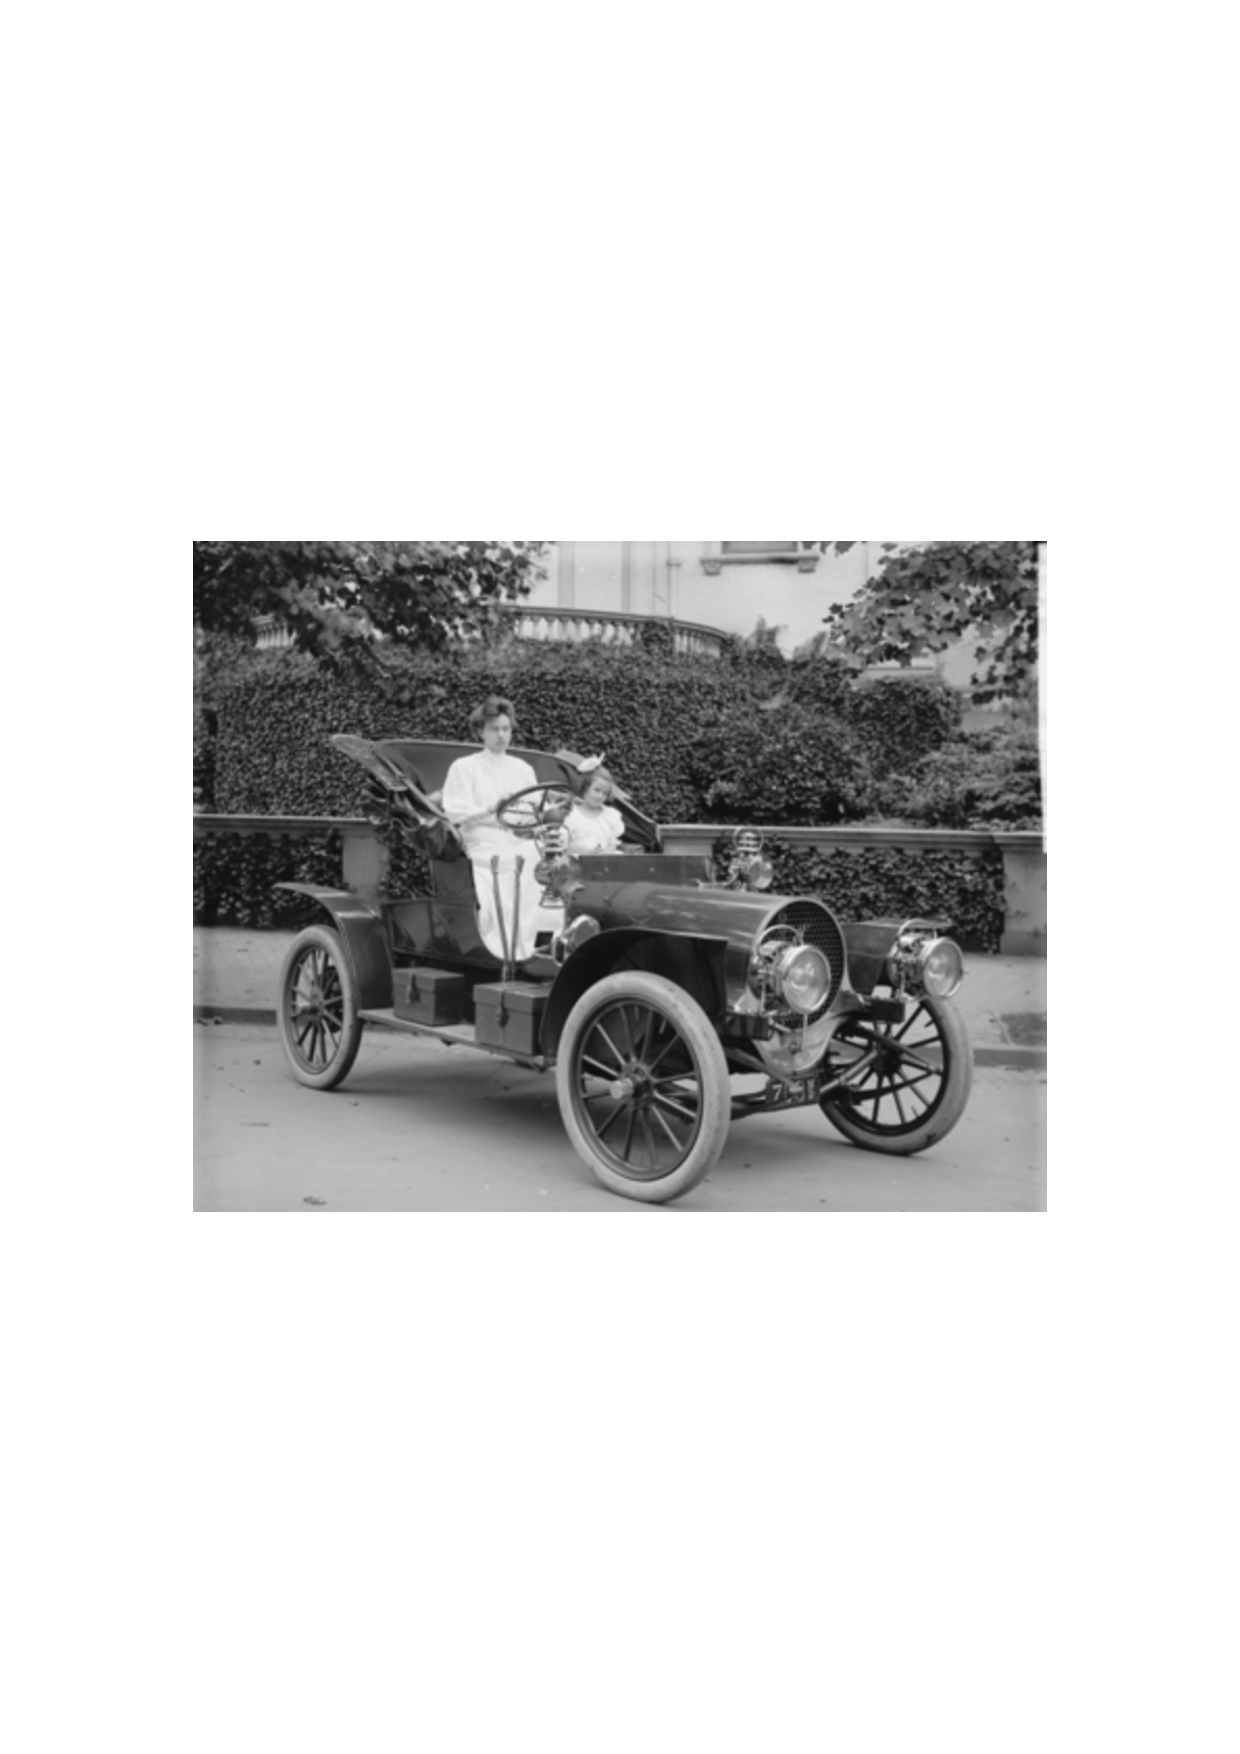
\includegraphics[width=0.8\linewidth]{figure/sample.pdf}
  \caption{1907 Franklin Model D roadster. Photograph by Harris \& Ewing, Inc. [Public domain], via Wikimedia Commons. (\url{https://goo.gl/VLCRBB}).}
  \label{fig:sample-figure}
\end{figure}

\subsection{Tables}

Put the caption above the table. Example of reference to Table~\ref{tab:sample-table}.

\begin{table}
  \caption{Frequency of Special Characters}
  \label{tab:sample-table}
  \centering
  \begin{tabular}{|c|c|l|}
    \toprule
    Non-English or Math&Frequency&Comments\\
    \midrule
    \O & 1 in 1,000& For Swedish names\\
    $\pi$ & 1 in 5& Common in math\\
    \$ & 4 in 5 & Used in business\\
    $\Psi^2_1$ & 1 in 40,000& Unexplained usage\\
  \bottomrule
\end{tabular}
\end{table}

See the \texttt{booktab} packaged documentation for further options.

\subsection{Bibliography}

Example of citations:
\begin{itemize}
	\item name: \citet{Salton1968}
	\item parenthesis: \citep{Salton1968}
\end{itemize}

An initial list of references is provided in the files \texttt{bibliography.bib} and \texttt{proceedings.bib} that you can expand.

See the \texttt{natbib} packaged documentation for further options.

\subsection{Acronyms}

Use the 

\begin{verbatim}
 \ac{acronym}
 \end{verbatim}

command to insert acronyms, eg. \ac{AP}. The command will expand the acronym the first time it is used.

An initial list of acronyms is provided in the file \texttt{acronyms.tex} that you can expand.

See the \texttt{acronym} packaged documentation for further options.


%% Define the bibliography file to be used
\bibliography{bibliography,proceedings}

\input{acronyms}


\end{document}
